\documentclass[a4]{article}
\usepackage{geometry}
\geometry{a4paper,left=2cm,right=3cm, top=2cm, bottom=2cm} 
%\usepackage[austrian]{babel}
\renewcommand{\familydefault}{\sfdefault}
\usepackage{amsfonts,latexsym,amssymb,graphicx}
\usepackage{subfigure,epsfig,epstopdf}
%\usepackage{pdfsync}
\usepackage[utf8]{inputenc}
%\usepackage[T1]{fontenc}
\usepackage{booktabs} % For professional looking tables
\usepackage{multirow}
\usepackage{amsmath}

\usepackage[section]{placeins}

\title{\bf 183.605 \\ Machine Learning for Visual Computing \\ Assignment 2}
\author{Group 12: \\
	Hanna Huber (0925230) \\ Lena Trautmann (1526567) \\ Elisabeth Wetzer (0726681)}
\date{\today}


\begin{document}
\maketitle
\noindent

\section{Assignment 2}
\subsection{The dual optimization problem}
Support Vector Machines, short SVM, maximize the distance between data points and the decision boundary, thereby cope with the common issue that new data points are easily misclassified if the decision boundary is located close to another data point. A linear decision boundary can be described by the equation $d(x)=w^T+w_0=0$ with a vector $w \in \mathbb{R}^d$ and $w_0 \in \mathbb{R}$. The distance of a point $x \in \mathbb{R}^d$ is given by $\frac{w^Tx+w_0}{||w||}$. Furthermore let $d(x_i)t_i>0$.
The distance to the decision boundary is to be maximized which leads to:
$$\frac{d(x_i)t_i}{||w||} \geq \tau$$
for $i \in \{1,2,..., N\}$ and $\tau >0$ the margin. Since the int hyperplane equation $d(x)=0$ $w$ as well as $w_0$ can be multiplied by a positive scalar without manipulating the solution, $\tau$ can be assumed as $\frac{1}{||w||}$.
The margin $\tau$ is maximized when the function $J=\frac{1}{2} ||w||^2$ is minimized under the constraints of $(w^Tx_i+w_0)t_i \geq1$.\\
This can be archieved by using Lagrange multipliers, leading to the formulation:\\
Maximize:
 $$L(\alpha)=-\frac{1}{2} \sum_{i,j=1}^N \alpha_i \alpha_j t_i t_j (x_i^T x_j) + \sum_{i=1}^N \alpha_i$$
 
 under the constraints $\alpha_i >0 \quad \forall i$ and $\sum_{i=1}^N \alpha_i t_i =0$.\\
 
 In other notation it can be expressed as minimizing:
 $$-L(\alpha)=\frac{1}{2} \alpha^T H \alpha + f^T \alpha$$

\noindent {\bf Tasks:}
\begin{itemize}
\item Generate a suitable training set of linearly separable data
\end{itemize}
The training set is generated in \texttt{generateTrainingData.m}. The function \texttt{generateTrainingData(N, xRange, yRange, linear)} takes the number of sample points, the domains (defined by a lower and an upper bound) from which the $x$ and $y$ coordinates are sampled and a flag which indicates if the resulting data should be linearly separable. A set of random 2D coordinates is created using the MATLAB function \texttt{rand}. Linear separability is achieved by labelling the according to the condition $ x_i + y_i > \bar{x} + \bar{y}$, where $\bar{x}$ and $\bar{y}$ denote the domain centers.

\begin{itemize}
\item Plot the input vectors in $\mathbb{R}^2$ and visualize corresponding target values (e.g. by using color). 
\end{itemize}
The resulting training data is displayed in Figure~\ref{fig:linearData}. Sample points with class label 1 are marked red, points with label -1 are merked green.
\begin{figure}[!h]
	\begin{center}
		\centering
		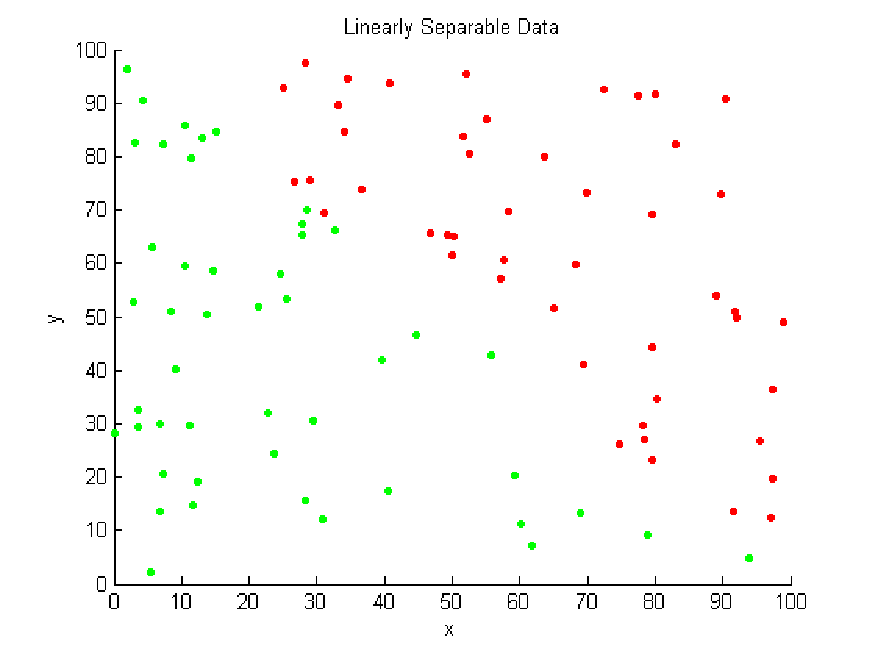
\includegraphics[width=6cm]{../figures/linearData.pdf}
	\end{center}	
	\caption{Linearly separable data with color-coded class labels (1=red, -1=green) for $N=100$.}
	\label{fig:linearData}
\end{figure}

\begin{itemize}
\item Visualize the support vectors and plot the decision boundary.
\end{itemize}
Figure~\ref{fig:sv} shows the support vectors defined by \texttt{trainSVM}.
\begin{figure}[!h]
	\begin{center}
		\centering
		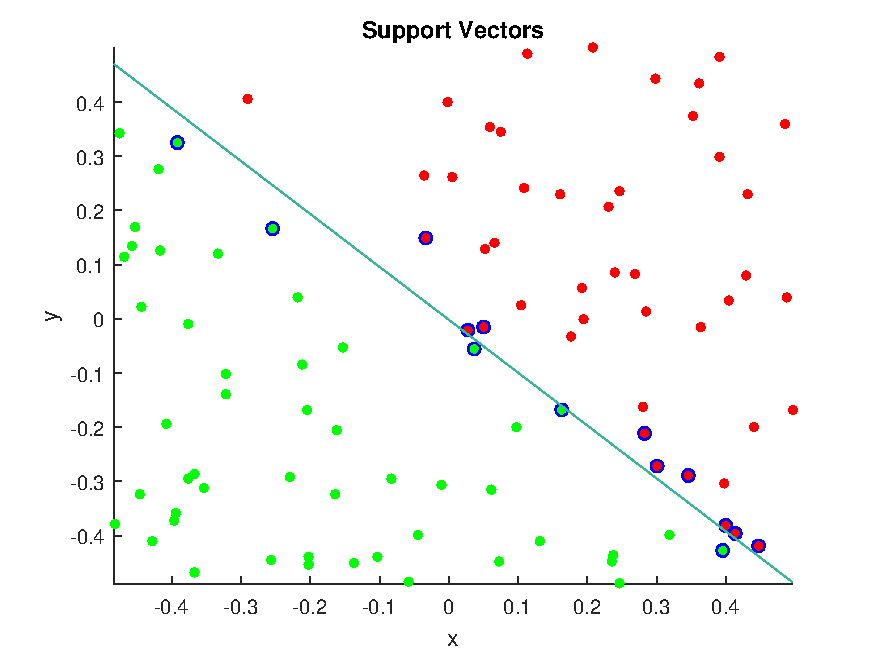
\includegraphics[width=6cm]{../figures/sv.pdf}
	\end{center}
	\caption{Training data with support vectors marked by blue circles and decision boundary plotted in blue.}
	\label{fig:sv}
\end{figure}


\subsection{The kernel trick}

\noindent {\bf Tasks:}
\begin{itemize}
\item Try different values for $\sigma$ (the RBF parameter).
\end{itemize}
\begin{figure}[h!]
\centering
	\subfigure[$\sigma=0.5$]{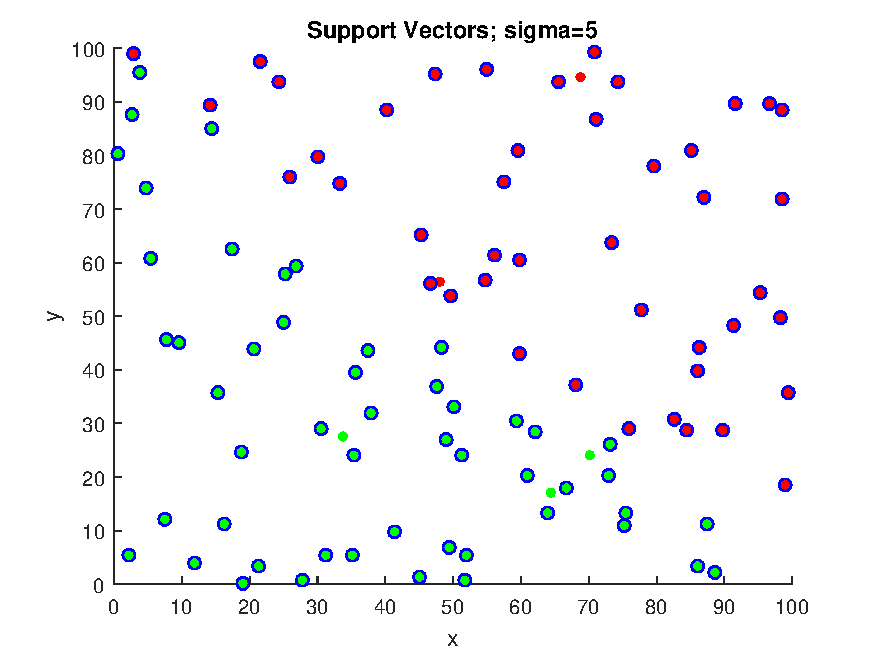
\includegraphics[width=5cm]{../figures/sv_kernel5.pdf}}
	\subfigure[$\sigma=0.15$]{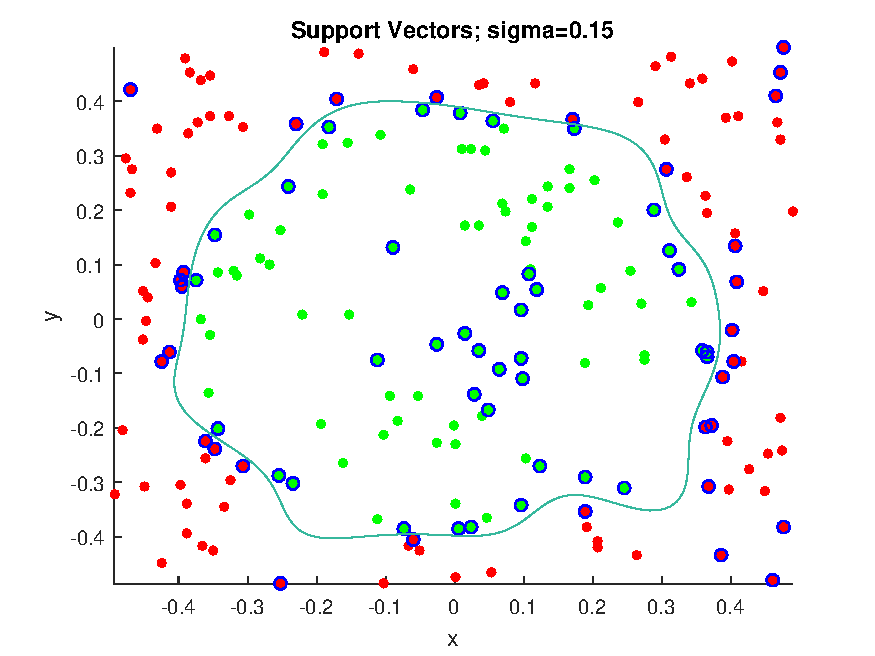
\includegraphics[width=5cm]{../figures/sv_kernel15.pdf}}
	\subfigure[$\sigma=0.25$]{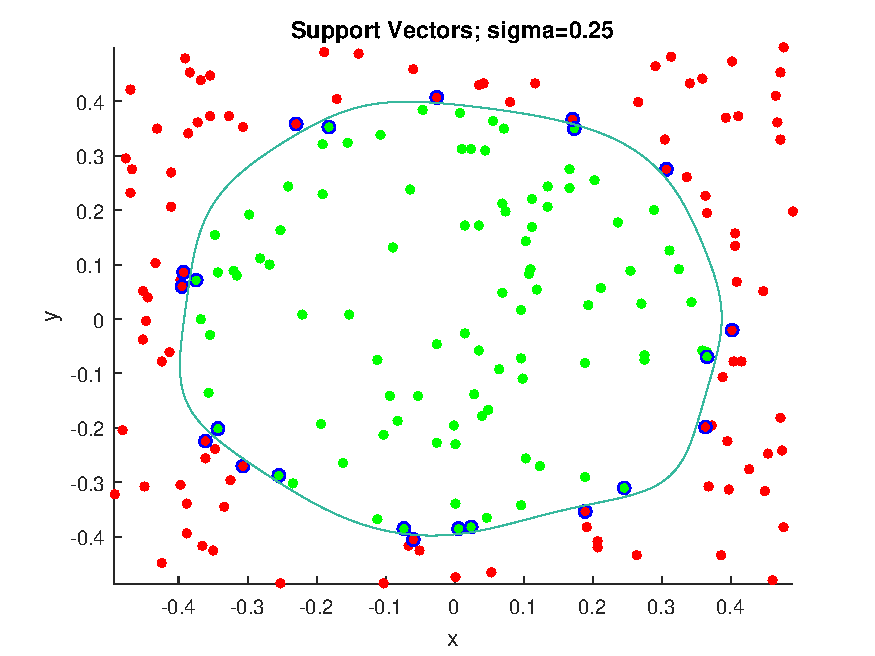
\includegraphics[width=5cm]{../figures/sv_kernel25.pdf}}
	\\
	\subfigure[$\sigma=0.35$]{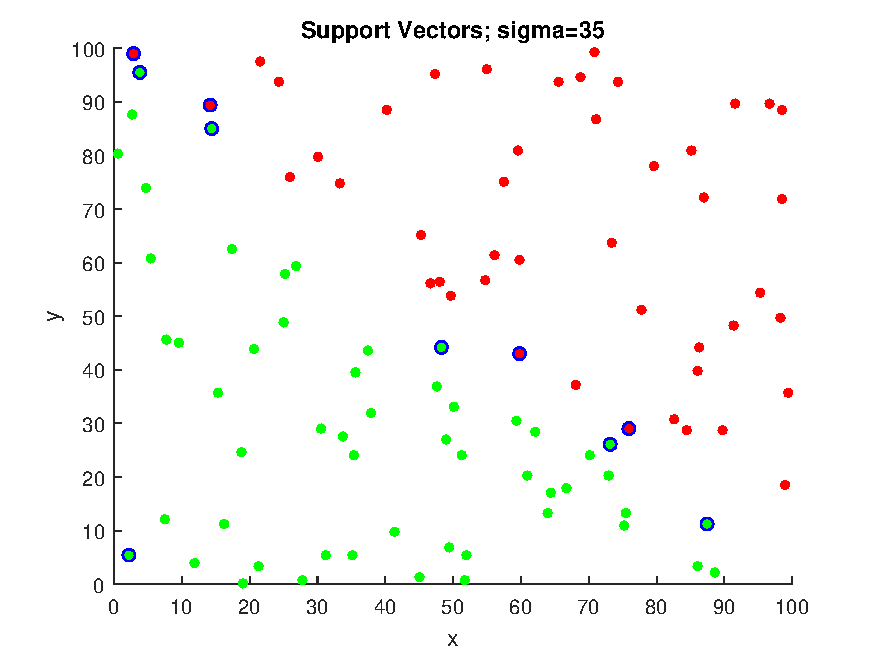
\includegraphics[width=5cm]{../figures/sv_kernel35.pdf}}
	\subfigure[$\sigma=0.45$]{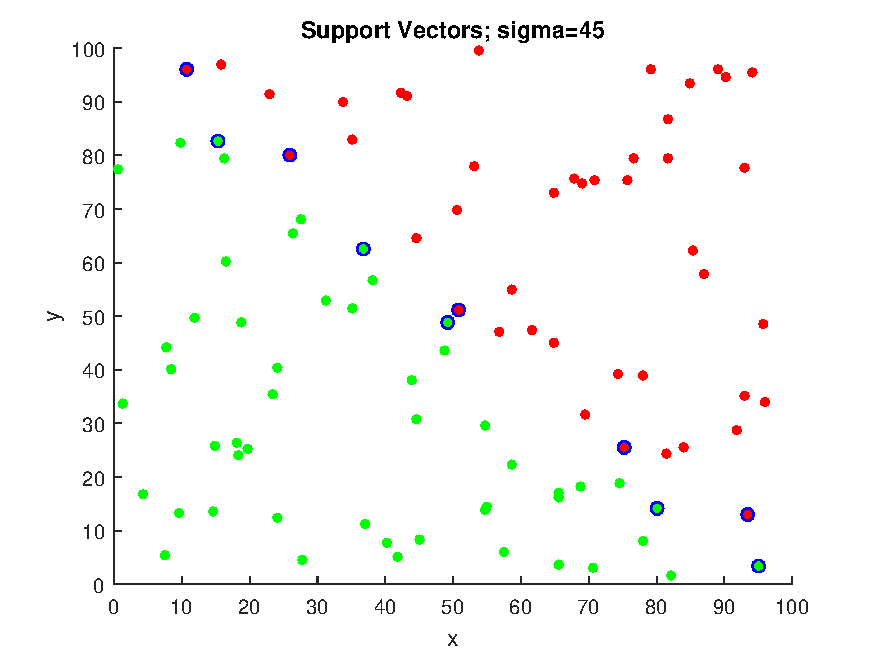
\includegraphics[width=5cm]{../figures/sv_kernel45.pdf}}
	\subfigure[$\sigma=0.55$]{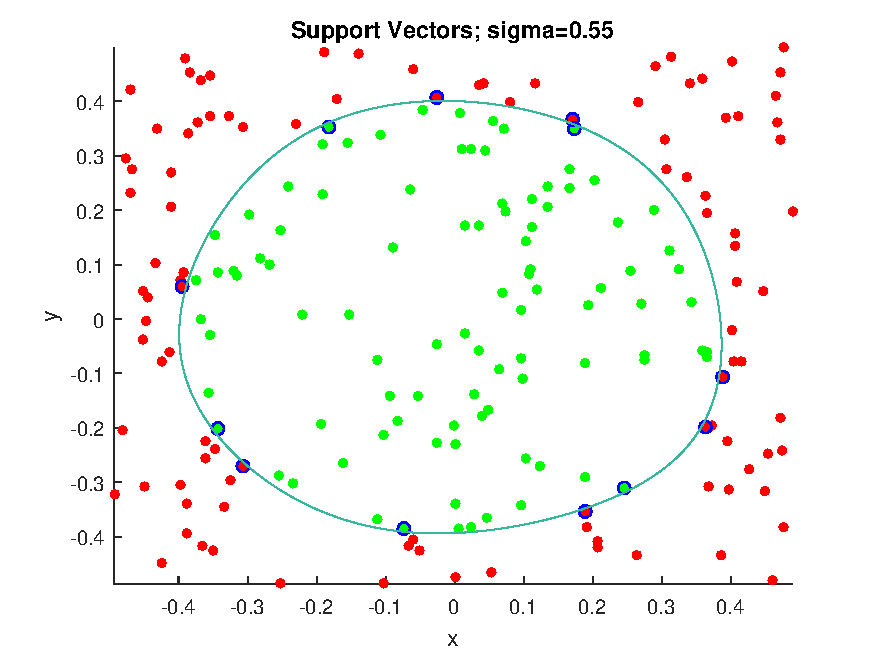
\includegraphics[width=5cm]{../figures/sv_kernel55.pdf}}
\caption{Training data with support vectors marked by blue circles and decision boundary plotted in blue, for different values of the RBF parameter $\sigma$.}
\label{fig:sv_kernel}
\end{figure}
The radial basis function kernel is defined by $K(x,y) = exp(-\frac{\|x-y\|^2}{\sigma^2})$.
The corresponding support vectors are shown in Figure~\ref{fig:sv_kernel} for different values of the RBF parameter $\sigma$. In the lecture notes about RBF-networks, we discussed a selection of $\sigma= 2*avgdist$, where $avgdist$ denotes the average distance of the centers. Having distances between the data points of approximately 10 units (or slightly more), $\sigma= 25$ is then selected.
% @Lena, Sigma=25?? 

\begin{itemize}
\item Generate a non-linearly separable training set, plot the data, visualize the support vectors and plot the decision boundary.
\end{itemize}
%See also Figure~\ref{fig:sv}
Figure \ref{fig:sv_kernel} shows that the decision boundaries for different values of $\sigma$, but the same non-linear seperable data set. It can be observed that a varying $\sigma$ leads to a varying number of support vectors.
%\begin{figure}[h!]
%\centering
%	\subfigure[]{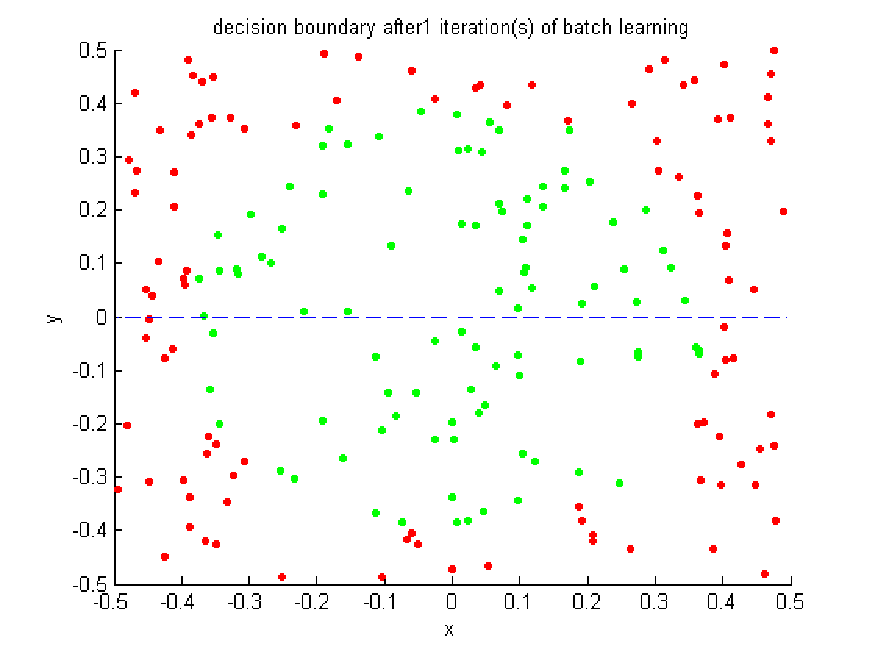
\includegraphics[width=5cm]{../figures/originalBatchIt1.pdf}}
%	\subfigure[]{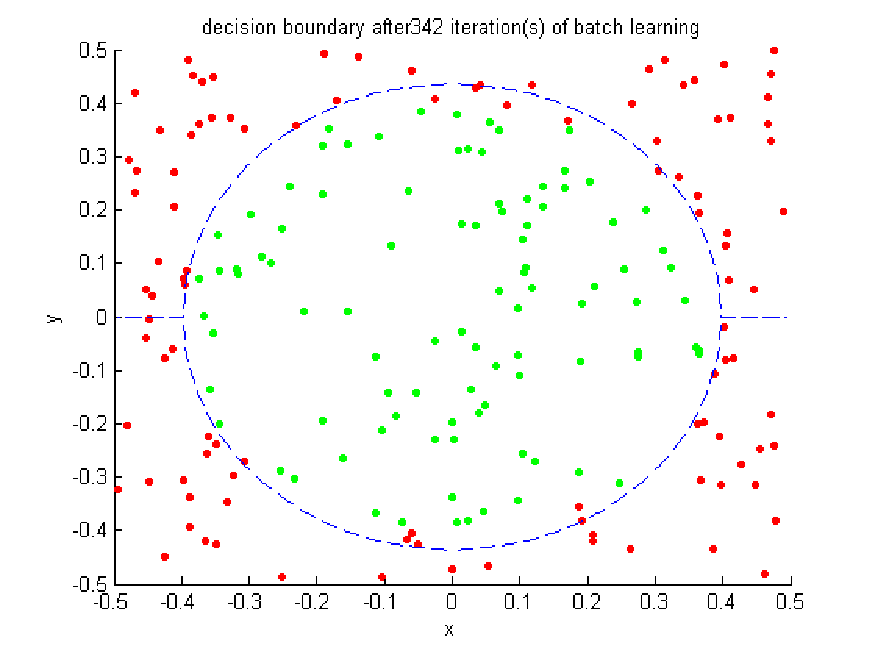
\includegraphics[width=5cm]{../figures/originalBatchIt342.pdf}}
%	\subfigure[]{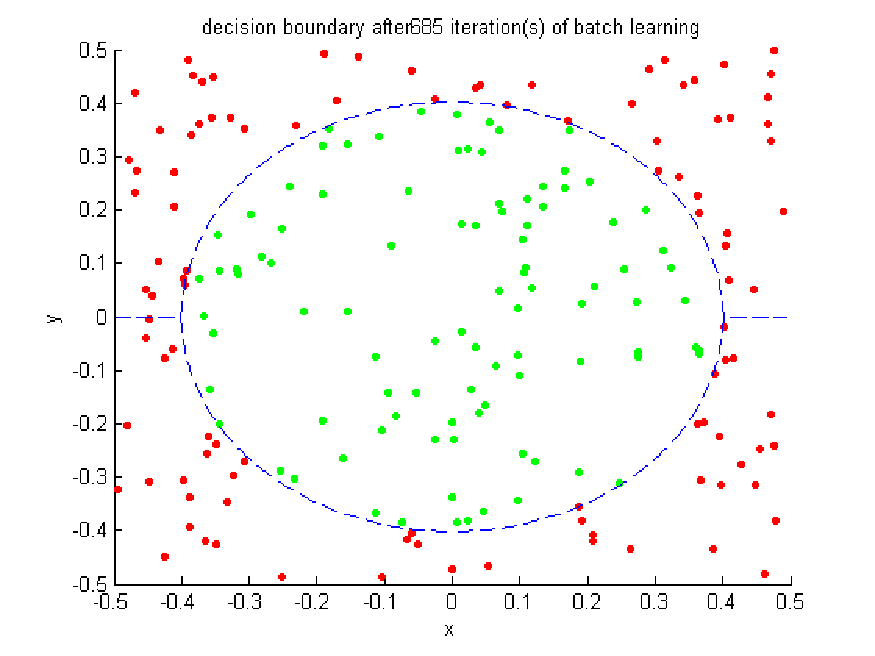
\includegraphics[width=5cm]{../figures/originalBatchIt685.pdf}}
%\caption{Perceptron decision boundary in the original data space at iterations \#1, \#342 and \#685 of batch learning.}
%\label{fig:origBA}
%\end{figure}


To train the non-linear seperable data using a RBF kernel using a slack variable $C$, we introduce an upper boundary for the Lagrange multipliers $\alpha _i$. The upper boundary is given by $\frac{C}{N}$. The value of the slack variables needs to be chosen carefully to prevent overfitting in case of large slack variables but may be chosen large enough to provide accurate SVM calculations.

% \bibliography{lit}
% \bibliographystyle{unsrt}

\end{document}
